\documentclass{lab1-article}

\title{Pendolo quadrifilare}

\newcommand{\plasduinodoctext}[1]%
{
  Una volta acceso il calcolatore, selezionare dal men\`u principale
  (in alto a sinistra) \menuitem{Application}~$\rightarrow$~%
  \menuitem{Education}~$\rightarrow$~\menuitem{plasduino}. Questo dovrebbe
  mostrare la finestra principale del programma di acquisizione. Per questa
  esperienza, tra la lista dei moduli, lanciate~\menuitem{#1} (doppio
  click sulla linea corrispondente, oppure selezionate la linea stessa e
  premete \menuitem{Open}).
}


\newcommand{\plasduinodoc}[1]%
{
  \labsection{Note sul programma di acquisizione}

  \plasduinodoctext{#1}
}

\newcommand{\plasduinosave}%
{
  Di norma al termine di ogni sessione di presa dati il programma vi chiede se
  volete salvare una copia del \emph{file} dei dati in una cartella a vostra
  scelta (il che pu\`o essere comodo per l'analisi successiva). Se questa
  funzionalit\`a dovesse essere disabilitata potete ri-abilitarla 
  attraverso il men\`u di plasduino \menuitem{Configuration}~%
  $\rightarrow$~\menuitem{Change settings}: nella finestra che si apre
  selezionate il tab~\menuitem{daq} e abilitate l'opzione
  \menuitem{prompt-save-dialog}.
}

\makeatletter
\def\PY@reset{\let\PY@it=\relax \let\PY@bf=\relax%
    \let\PY@ul=\relax \let\PY@tc=\relax%
    \let\PY@bc=\relax \let\PY@ff=\relax}
\def\PY@tok#1{\csname PY@tok@#1\endcsname}
\def\PY@toks#1+{\ifx\relax#1\empty\else%
    \PY@tok{#1}\expandafter\PY@toks\fi}
\def\PY@do#1{\PY@bc{\PY@tc{\PY@ul{%
    \PY@it{\PY@bf{\PY@ff{#1}}}}}}}
\def\PY#1#2{\PY@reset\PY@toks#1+\relax+\PY@do{#2}}

\expandafter\def\csname PY@tok@gd\endcsname{\def\PY@tc##1{\textcolor[rgb]{0.63,0.00,0.00}{##1}}}
\expandafter\def\csname PY@tok@gu\endcsname{\let\PY@bf=\textbf\def\PY@tc##1{\textcolor[rgb]{0.50,0.00,0.50}{##1}}}
\expandafter\def\csname PY@tok@gt\endcsname{\def\PY@tc##1{\textcolor[rgb]{0.00,0.27,0.87}{##1}}}
\expandafter\def\csname PY@tok@gs\endcsname{\let\PY@bf=\textbf}
\expandafter\def\csname PY@tok@gr\endcsname{\def\PY@tc##1{\textcolor[rgb]{1.00,0.00,0.00}{##1}}}
\expandafter\def\csname PY@tok@cm\endcsname{\let\PY@it=\textit\def\PY@tc##1{\textcolor[rgb]{0.25,0.50,0.50}{##1}}}
\expandafter\def\csname PY@tok@vg\endcsname{\def\PY@tc##1{\textcolor[rgb]{0.10,0.09,0.49}{##1}}}
\expandafter\def\csname PY@tok@m\endcsname{\def\PY@tc##1{\textcolor[rgb]{0.40,0.40,0.40}{##1}}}
\expandafter\def\csname PY@tok@mh\endcsname{\def\PY@tc##1{\textcolor[rgb]{0.40,0.40,0.40}{##1}}}
\expandafter\def\csname PY@tok@go\endcsname{\def\PY@tc##1{\textcolor[rgb]{0.53,0.53,0.53}{##1}}}
\expandafter\def\csname PY@tok@ge\endcsname{\let\PY@it=\textit}
\expandafter\def\csname PY@tok@vc\endcsname{\def\PY@tc##1{\textcolor[rgb]{0.10,0.09,0.49}{##1}}}
\expandafter\def\csname PY@tok@il\endcsname{\def\PY@tc##1{\textcolor[rgb]{0.40,0.40,0.40}{##1}}}
\expandafter\def\csname PY@tok@cs\endcsname{\let\PY@it=\textit\def\PY@tc##1{\textcolor[rgb]{0.25,0.50,0.50}{##1}}}
\expandafter\def\csname PY@tok@cp\endcsname{\def\PY@tc##1{\textcolor[rgb]{0.74,0.48,0.00}{##1}}}
\expandafter\def\csname PY@tok@gi\endcsname{\def\PY@tc##1{\textcolor[rgb]{0.00,0.63,0.00}{##1}}}
\expandafter\def\csname PY@tok@gh\endcsname{\let\PY@bf=\textbf\def\PY@tc##1{\textcolor[rgb]{0.00,0.00,0.50}{##1}}}
\expandafter\def\csname PY@tok@ni\endcsname{\let\PY@bf=\textbf\def\PY@tc##1{\textcolor[rgb]{0.60,0.60,0.60}{##1}}}
\expandafter\def\csname PY@tok@nl\endcsname{\def\PY@tc##1{\textcolor[rgb]{0.63,0.63,0.00}{##1}}}
\expandafter\def\csname PY@tok@nn\endcsname{\let\PY@bf=\textbf\def\PY@tc##1{\textcolor[rgb]{0.00,0.00,1.00}{##1}}}
\expandafter\def\csname PY@tok@no\endcsname{\def\PY@tc##1{\textcolor[rgb]{0.53,0.00,0.00}{##1}}}
\expandafter\def\csname PY@tok@na\endcsname{\def\PY@tc##1{\textcolor[rgb]{0.49,0.56,0.16}{##1}}}
\expandafter\def\csname PY@tok@nb\endcsname{\def\PY@tc##1{\textcolor[rgb]{0.00,0.50,0.00}{##1}}}
\expandafter\def\csname PY@tok@nc\endcsname{\let\PY@bf=\textbf\def\PY@tc##1{\textcolor[rgb]{0.00,0.00,1.00}{##1}}}
\expandafter\def\csname PY@tok@nd\endcsname{\def\PY@tc##1{\textcolor[rgb]{0.67,0.13,1.00}{##1}}}
\expandafter\def\csname PY@tok@ne\endcsname{\let\PY@bf=\textbf\def\PY@tc##1{\textcolor[rgb]{0.82,0.25,0.23}{##1}}}
\expandafter\def\csname PY@tok@nf\endcsname{\def\PY@tc##1{\textcolor[rgb]{0.00,0.00,1.00}{##1}}}
\expandafter\def\csname PY@tok@si\endcsname{\let\PY@bf=\textbf\def\PY@tc##1{\textcolor[rgb]{0.73,0.40,0.53}{##1}}}
\expandafter\def\csname PY@tok@s2\endcsname{\def\PY@tc##1{\textcolor[rgb]{0.73,0.13,0.13}{##1}}}
\expandafter\def\csname PY@tok@vi\endcsname{\def\PY@tc##1{\textcolor[rgb]{0.10,0.09,0.49}{##1}}}
\expandafter\def\csname PY@tok@nt\endcsname{\let\PY@bf=\textbf\def\PY@tc##1{\textcolor[rgb]{0.00,0.50,0.00}{##1}}}
\expandafter\def\csname PY@tok@nv\endcsname{\def\PY@tc##1{\textcolor[rgb]{0.10,0.09,0.49}{##1}}}
\expandafter\def\csname PY@tok@s1\endcsname{\def\PY@tc##1{\textcolor[rgb]{0.73,0.13,0.13}{##1}}}
\expandafter\def\csname PY@tok@sh\endcsname{\def\PY@tc##1{\textcolor[rgb]{0.73,0.13,0.13}{##1}}}
\expandafter\def\csname PY@tok@sc\endcsname{\def\PY@tc##1{\textcolor[rgb]{0.73,0.13,0.13}{##1}}}
\expandafter\def\csname PY@tok@sx\endcsname{\def\PY@tc##1{\textcolor[rgb]{0.00,0.50,0.00}{##1}}}
\expandafter\def\csname PY@tok@bp\endcsname{\def\PY@tc##1{\textcolor[rgb]{0.00,0.50,0.00}{##1}}}
\expandafter\def\csname PY@tok@c1\endcsname{\let\PY@it=\textit\def\PY@tc##1{\textcolor[rgb]{0.25,0.50,0.50}{##1}}}
\expandafter\def\csname PY@tok@kc\endcsname{\let\PY@bf=\textbf\def\PY@tc##1{\textcolor[rgb]{0.00,0.50,0.00}{##1}}}
\expandafter\def\csname PY@tok@c\endcsname{\let\PY@it=\textit\def\PY@tc##1{\textcolor[rgb]{0.25,0.50,0.50}{##1}}}
\expandafter\def\csname PY@tok@mf\endcsname{\def\PY@tc##1{\textcolor[rgb]{0.40,0.40,0.40}{##1}}}
\expandafter\def\csname PY@tok@err\endcsname{\def\PY@bc##1{\setlength{\fboxsep}{0pt}\fcolorbox[rgb]{1.00,0.00,0.00}{1,1,1}{\strut ##1}}}
\expandafter\def\csname PY@tok@kd\endcsname{\let\PY@bf=\textbf\def\PY@tc##1{\textcolor[rgb]{0.00,0.50,0.00}{##1}}}
\expandafter\def\csname PY@tok@ss\endcsname{\def\PY@tc##1{\textcolor[rgb]{0.10,0.09,0.49}{##1}}}
\expandafter\def\csname PY@tok@sr\endcsname{\def\PY@tc##1{\textcolor[rgb]{0.73,0.40,0.53}{##1}}}
\expandafter\def\csname PY@tok@mo\endcsname{\def\PY@tc##1{\textcolor[rgb]{0.40,0.40,0.40}{##1}}}
\expandafter\def\csname PY@tok@kn\endcsname{\let\PY@bf=\textbf\def\PY@tc##1{\textcolor[rgb]{0.00,0.50,0.00}{##1}}}
\expandafter\def\csname PY@tok@mi\endcsname{\def\PY@tc##1{\textcolor[rgb]{0.40,0.40,0.40}{##1}}}
\expandafter\def\csname PY@tok@gp\endcsname{\let\PY@bf=\textbf\def\PY@tc##1{\textcolor[rgb]{0.00,0.00,0.50}{##1}}}
\expandafter\def\csname PY@tok@o\endcsname{\def\PY@tc##1{\textcolor[rgb]{0.40,0.40,0.40}{##1}}}
\expandafter\def\csname PY@tok@kr\endcsname{\let\PY@bf=\textbf\def\PY@tc##1{\textcolor[rgb]{0.00,0.50,0.00}{##1}}}
\expandafter\def\csname PY@tok@s\endcsname{\def\PY@tc##1{\textcolor[rgb]{0.73,0.13,0.13}{##1}}}
\expandafter\def\csname PY@tok@kp\endcsname{\def\PY@tc##1{\textcolor[rgb]{0.00,0.50,0.00}{##1}}}
\expandafter\def\csname PY@tok@w\endcsname{\def\PY@tc##1{\textcolor[rgb]{0.73,0.73,0.73}{##1}}}
\expandafter\def\csname PY@tok@kt\endcsname{\def\PY@tc##1{\textcolor[rgb]{0.69,0.00,0.25}{##1}}}
\expandafter\def\csname PY@tok@ow\endcsname{\let\PY@bf=\textbf\def\PY@tc##1{\textcolor[rgb]{0.67,0.13,1.00}{##1}}}
\expandafter\def\csname PY@tok@sb\endcsname{\def\PY@tc##1{\textcolor[rgb]{0.73,0.13,0.13}{##1}}}
\expandafter\def\csname PY@tok@k\endcsname{\let\PY@bf=\textbf\def\PY@tc##1{\textcolor[rgb]{0.00,0.50,0.00}{##1}}}
\expandafter\def\csname PY@tok@se\endcsname{\let\PY@bf=\textbf\def\PY@tc##1{\textcolor[rgb]{0.73,0.40,0.13}{##1}}}
\expandafter\def\csname PY@tok@sd\endcsname{\let\PY@it=\textit\def\PY@tc##1{\textcolor[rgb]{0.73,0.13,0.13}{##1}}}

\def\PYZbs{\char`\\}
\def\PYZus{\char`\_}
\def\PYZob{\char`\{}
\def\PYZcb{\char`\}}
\def\PYZca{\char`\^}
\def\PYZam{\char`\&}
\def\PYZlt{\char`\<}
\def\PYZgt{\char`\>}
\def\PYZsh{\char`\#}
\def\PYZpc{\char`\%}
\def\PYZdl{\char`\$}
\def\PYZhy{\char`\-}
\def\PYZsq{\char`\'}
\def\PYZdq{\char`\"}
\def\PYZti{\char`\~}
% for compatibility with earlier versions
\def\PYZat{@}
\def\PYZlb{[}
\def\PYZrb{]}
\makeatother


\begin{document}


\begin{article}
\selectlanguage{italian}

\maketitle

\secsummary
L'esperienza verte sullo studio del moto di un pendolo e della dipendenza del
periodo dall'ampiezza dell'oscillazione.

\secmaterials

\begin{itemize}
\item Un pendolo quadrifilare;
\item metro a nastro (risoluzione 1~mm);
\item un computer per acquisizione ed analisi dei dati.
\end{itemize}

\secdefinitions

\begin{figure}[htb!]
  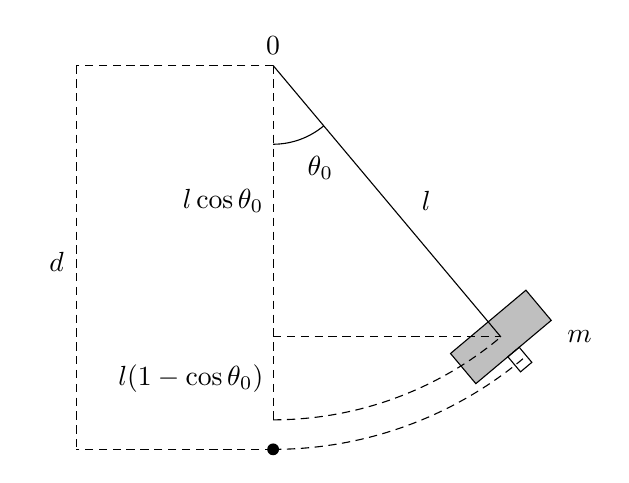
\begin{tikzpicture}[scale=1]
    \pgfmathsetmacro{\xc}{3}
    \pgfmathsetmacro{\yc}{0}
    \pgfmathsetmacro{\r}{4.5}
    \pgfmathsetmacro{\w}{1.25}
    \pgfmathsetmacro{\h}{0.5}
    \pgfmathsetmacro{\doff}{2.5}
    \pgfmathsetmacro{\rangle}{1}
    \pgfmathsetmacro{\thetazero}{40}
    \node at (0, 0) {};
    \fill[draw=black, fill=lightgray, rotate around={\thetazero:(\xc, \yc)}]%
    (\xc - 0.5*\w, \yc - \r - 0.5*\h) rectangle%
    (\xc + 0.5*\w, \yc - \r + 0.5*\h);
    \draw[rotate around={\thetazero:(\xc, \yc)}]%
    (\xc - 0.075*\w, \yc - \r - 0.5*\h) rectangle%
    (\xc + 0.075*\w, \yc - \r - \h);
    \fill (\xc, \yc - \r - 0.75*\h) circle [radius=0.075];
    \draw[style=densely dashed] (\xc, \yc) -- (\xc, \yc - \r);
    \draw[style=densely dashed] (\xc, \yc - \r - 0.75*\h) --%
    (\xc - \doff, \yc - \r - 0.75*\h);
    \draw[style=densely dashed] (\xc, \yc) -- (\xc - \doff, \yc);
    \draw[style=densely dashed] (\xc - \doff, \yc) --%
    (\xc - \doff, \yc - \r -0.75*\h);
    \node at (\xc - \doff - 0.25, \yc - 0.5*\r - 0.5*\h) {$d$};

    \draw (\xc, \yc) -- (\xc + \r*sin{\thetazero}, \yc - \r*cos{\thetazero});
    \draw[style=densely dashed] (\xc, \yc - \r) arc (270:270+\thetazero:\r);
    \draw[style=densely dashed] (\xc, \yc - \r - 0.75*\h) arc%
    (270:270+\thetazero:1.1*\r);
    \draw[style=densely dashed] (\xc, \yc - \r*cos{\thetazero}) --%
    (\xc + \r*sin{\thetazero}, \yc - \r*cos{\thetazero});
    \draw (\xc, \yc - \rangle) arc (270:270+\thetazero:\rangle);
    \node at (\xc, \yc + 0.25) {$0$};
    \node[anchor=east] at (\xc , \yc - 0.5*\r*cos{\thetazero})%
         {$l\cos\theta_0$};
    \node[anchor=east] at (\xc , \yc - 0.5*\r - 0.5*\r*cos{\thetazero})%
         {$l (1 - \cos\theta_0)$};
    \node at (\xc + 0.5*\r*sin{\thetazero} + 0.5, \yc - 0.5*\r*cos{\thetazero})%
          {$l$};
    \node at (\xc + 0.6, \yc - 1.3) {$\theta_0$};
    \node at (\xc + \r*sin{\thetazero} + 1, \yc - \r*cos{\thetazero}) {$m$};
  \end{tikzpicture}
  \caption{Schematizzazione dell'apparato sperimentale e definizioni di base.}
  \label{fig:pendolo}
\end{figure}

Al di l\`a delle definizioni ovvie, sottolineiamo la differenza tra la lunghezza
$l$ del pendolo e la distanza $d$ tra il punto di sospensione ed il traguardo
ottico che registra i passaggi della bandierina.

Ricordiamo inoltre che l'espressione per il periodo del pendolo si pu\`o
sviluppare in serie come
\begin{align}\label{eq:pendulum_taylor}
T = 2\pi\sqrt{\frac{l}{g}} \left( 1 + \frac{1}{16}\theta_0^2 +
\frac{11}{3072}\theta_0^4 + \cdots \right).
\end{align}


\secmeasurements

Nel momento in cui il pendolo si trova (con velocit\`a nulla) nella posizione
di massima altezza raggiunta dall'\mbox{i-esima} oscillazione la sua energia meccanica
sar\`a soltanto energia potenziale. Al contrario, nel punto pi\`u basso della
traiettoria (a patto di fissare opportunamente lo zero del potenziale), si
avr\`a solamente energia cinetica.


\labsubsection{Misure di velocit\`a}

Si costruisca il grafico della velocit\`a $v_0$ nel punto pi\`u basso in
funzione del tempo. Nel caso di smorzamento proporzionale alla velocit\`a
ci si aspetta un andamento esponenziale:
\begin{align}
  v_0(t) = v_0(0) e^{-\lambda t}.
\end{align}
Si stimi, tramite un fit, la costante di smorzamento
$\lambda$ e il tempo di smorzamento associato $\tau = 1/\lambda$.

Per completezza, pu\`o essere interessante costruire il grafico cartesiano
del periodo $T$ in funzione del tempo. A causa della variazione dell'ampiezza
di oscillazione, anch'esso diminuir\`a nel tempo.


\labsubsection{Misure di smorzamento}

L'ampiezza \emph{(quasi) istantanea} di oscillazione si pu\`o ricavare,
assumendo trascurabile la perdita di energia per attrito su un quarto di periodo, dal
bilancio energetico
\begin{align}
  mgl(1 - \cos\theta_0) = \frac{1}{2}mv_0^2,
\end{align}
da cui si ricava banalmente
\begin{align}
  \theta_0 = \arccos\left( 1 - \frac{v_0^2}{2gl} \right).
\end{align}

Si costruisca il grafico cartesiano del periodo $T$ in funzione
dell'ampiezza $\theta_0$ di oscillazione  e si verifichi
la~\eqref{eq:pendulum_taylor}.
Quanti ordini dello sviluppo in serie si riescono a \emph{vedere}?


\secconsiderations

\subsecdataformat

Il programma di acquisizione registra il tempo di ogni transizione
dello del traguardo ottico, e fornisce un \emph{file} di uscita contenente tre
colonne che rappresentano, rispettivamente:
\begin{enumerate}
\item il tempo dall'inizio della presa dati;
\item il periodo $T$ dell'oscillazione corrente;
\item il tempo di transito $t_{\rm T}$ della bandierina.
\end{enumerate}

Detta $w$ la larghezza della bandierina, la velocit\`a del centro di massa del
pendolo nel punto pi\`u basso dell'oscillazione si ottiene come
\begin{align}
  v_0 = \frac{w}{t_{\rm T}} \times \frac{l}{d}
\end{align}
%(si faccia riferimento alla figura per convincersi che la velocit\`a del
%centro di massa \`e leggermente pi\`u piccola---di un fattore $l/d$, per la
%precisione---della velocit\`a della badierina).


\onecolumn

\plasduinodoc{Pendulum}

\plasduinosave


\end{article}
\end{document}
